\documentclass[letterpaper,10pt]{article}

\usepackage{titling}
\usepackage{listings}
\usepackage{url}
\usepackage{setspace}
\usepackage{subfig}
\usepackage{sectsty}
\usepackage{pdfpages}
\usepackage{colortbl}
\usepackage{multirow}
\usepackage{multicol}
\usepackage{relsize}
\usepackage{amsmath}
\usepackage{fancyvrb}
\usepackage{amsmath,amssymb,amsthm,graphicx,xspace}
\usepackage[titlenotnumbered,noend,noline]{algorithm2e}
\usepackage[compact]{titlesec}
\usepackage{XCharter}
\usepackage[T1]{fontenc}
\usepackage{tikz}
\usetikzlibrary{arrows,automata,shapes,trees,matrix,chains,scopes,positioning,calc}
\tikzstyle{block} = [rectangle, draw, fill=blue!20, 
    text width=2.5em, text centered, rounded corners, minimum height=2em]
\tikzstyle{bw} = [rectangle, draw, fill=blue!20, 
    text width=4em, text centered, rounded corners, minimum height=2em]

\newcommand{\CPP}{C\nolinebreak\hspace{-.05em}\raisebox{.4ex}{\tiny\bf +}\nolinebreak\hspace{-.10em}\raisebox{.4ex}{\tiny\bf +}}
\def\CPP{{C\nolinebreak[4]\hspace{-.05em}\raisebox{.4ex}{\tiny\bf ++}}}

\let\LaTeXtitle\title
\renewcommand{\title}[1]{\LaTeXtitle{\textsf{#1}}}


\addtolength{\oddsidemargin}{-1.000in}
\addtolength{\evensidemargin}{-0.500in}
\addtolength{\textwidth}{2.0in}
\addtolength{\topmargin}{-1.000in}
\addtolength{\textheight}{1.75in}
\addtolength{\parskip}{\baselineskip}
\setlength{\parindent}{0in}
\renewcommand{\baselinestretch}{1.5}

\singlespace

\begin{document}

\lecture{29 --- Profiling and Scalability}{\term}{Jeff Zarnett}

\section*{Profiling and Scalability}

Following the discussion of profiling, we should take some time to understand performance and scalability. Recall that what we want in scalability is that we can take our software from 1 user to 100 to 10 million. Finishing work faster helps, but it's not the only way. So to scale up, we probably need to do some profiling to find out what's slow, but we have some things we need to worry about when we want to get away from just working on our dev machines and into big numbers of users.

So we should respect the following principles, as outlined in~\cite{swps}.

\paragraph{Hardware Principle.} 
Scalability testing is very different from  QA testing (as if you actually test your code!) in that you will do development and QA on your local computer and all you really care about is whether the program produces the correct output ``fast enough''. That's fine, but it's no way to test if it scales. If you actually want to test for scalability and real world performance, you should be doing it on the machines that are going to run the program in the live environment. Why? Well, low-end systems have very different limiting factors. You might be limited by the 4GB of RAM in your laptop and that would go away in the 64GB of RAM server you're using. So you might spend a great deal of time worrying about RAM usage when it turns out it doesn't matter.

\paragraph{Reality Principle.}
It would be a good idea to use a ``real'' workload, as much as one can possibly simulate. Legal reasons might prevent you from using actual customer data, but you should be trying to use the best approximation of it that you have. If you only generate some test data, you may not accurately represent the way the users are going to behave the system. Your test set run summary reports occasionally... your users might run them every hour. 

\paragraph{Volume Principle.}
``More is the new more.'' It's okay to use lighter workloads for regression testing and things like that, but if you actually want to see how your system performs under pressure, you actually need to put it under pressure. You can simulate pressure by limiting RAM or running something very CPU-intensive concurrently, but it's just not the same.

These tests, incidentally, are of great interest to the customers, who would like to know that you can deliver. 

\paragraph{Reproducibility and Regression Testing.}
Your results will need to be reproducible. Remember that good programming practice says that unit tests should be run, and re-run to make sure it all works. The same is true in your performance tests. Just as we don't want to see old bugs cropping up again, old (solved) performance issues are not nice to see either. Or a new change that slows the whole program down is not a success either. So please, have regression testing and performance regression testing. Real-life example: \href{https://arewefastyet.com}{arewefastyet.com} tracks regressions/improvements in Firefox perf.

\section*{Characterizing Performance \& Scalability Problems}

\begin{quote}
\textit{It is a capital mistake to theorize before one has data. Insensibly one begins to twist facts to suit theories, instead of theories to suit facts.}
\end{quote}
\hfill - Sherlock Holmes (\textit{A Scandal in Bohemia}; Sir Arthur Conan Doyle)

Keeping the wisdom of Mr. Holmes in mind, we need to collect evidence before reaching conclusions. At a high level we probably have four potential culprits to start with:
\begin{enumerate}
	\item CPU
	\item Memory
	\item Disk
	\item Network
\end{enumerate}

These are, obviously, more categories than specific causes, but they are starting points for further investigation. They are listed in some numerical order, but there is no reason why one would have to investigate them in the order defined there.

CPU is probably the easiest of these to diagnose. Something like \texttt{top} or Task Manager will tell you pretty quickly if the CPU is busy. You can look at the \%CPU columns and see where all your CPU is going. Still, that tells you about right now; what about the long term average? Checking with my machine ``Loki'', that used to donate its free CPU cycles to world community grid (I'm singlehandedly saving the world, you see.):

\begin{verbatim}
top - 07:28:19 up 151 days, 23:38,  8 users,  load average: 0.87, 0.92, 0.91
\end{verbatim}

Those last three numbers are the one, five, and fifteen minute averages of CPU load, respectively. Lower numbers mean less CPU usage and a less busy machine. A small guide on how to interpret this, from~\cite{scout}.

Picture a single core of a CPU as a lane of traffic. You are a bridge operator and so you need to monitor how many cars are waiting to cross that bridge. If no cars are waiting, traffic is good and drivers are happy. If there is a backup of cars, then there will be delays. Our numbering scheme corresponds to this:

\begin{enumerate}
	\item 0.00 means no traffic (and in fact anything between 0.00 and 0.99) means we're under capacity and there will be no delay.
	\item 1.00 means we are exactly at capacity. Everything is okay, but if one more car shows up, there will be a delay.
	\item Anything above 1.00 means there's a backup (delay). If we have 2.00 load, then the bridge is full and there's an equal number of cars waiting to get on the bridge. 
\end{enumerate}

Or, visually, also from~\cite{scout}:

\begin{center}
	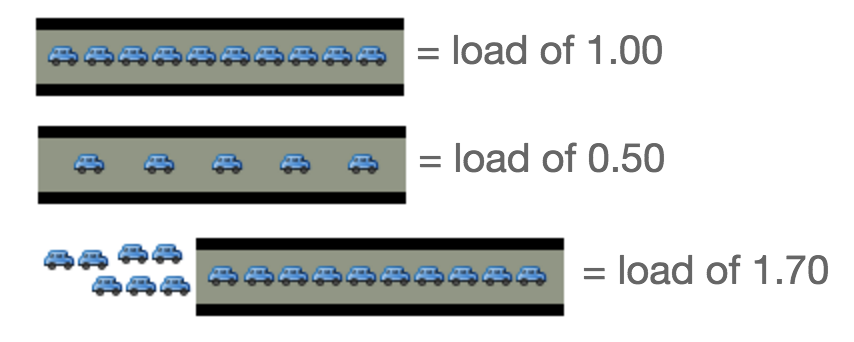
\includegraphics[width=0.55\textwidth]{images/car-analogy.png}
\end{center}

Being at or above 1.00 isn't necessarily bad, but you should be concerned if there is consistent load of 1.00 or above. And if you are below 1.00 but getting close to it, you know how much room you have to scale things up -- if load is 0.4 you can increase handily. If load is 0.9 you're pushing the limit already. If load is above 0.70 then it's probably time to investigate. If it's at 1.00 consistently we have a serious problem. If it's up to 5.00 then this is a red alert situation.

Now this is for a single CPU -- if you have a load of 3.00 and a quad core CPU, this is okay. You have, in the traffic analogy, four lanes of traffic, of which 3 are being used to capacity. So we have a fourth lane free and it's as if we're at 75\% utilization on a single CPU.


Next on the list is memory. One way to tell if memory is the limiting factor is actually to look at disk utilization. If there is not enough RAM in the box, there will be swapping and then performance goes out the window and scalability goes with. That is of course, the worst case. You can ask via \texttt{top} about how much swap is being used, but that's probably not the interesting value. 

\begin{verbatim}
KiB Mem:   8167736 total,  6754408 used,  1413328 free,   172256 buffers
KiB Swap:  8378364 total,  1313972 used,  7064392 free.  2084336 cached Mem
\end{verbatim}

This can be misleading though, because memory being ``full'' does not necessarily mean anything bad. It means the resource is being used to its maximum potential, yes, but there is no benefit to keeping a block of memory open for no reason. Things will move into and out of memory as they need to, and nobody hands out medals to indicate that you did an awesome job of keeping free memory. It's not like going under budget in your department for the year.  Also, memory is not like the CPU; if there's nothing for the CPU to do, it will just idle (or go to a low power state, which is nice for saving the planet). But memory won't ``forget'' data if it doesn't happen to be needed right now - data will hang around in memory until there is a reason to move or change it. So freaking out about memory appearing as full is kind of like getting all in a knot about how ``System Idle Process'' is hammering the CPU\footnote{Yes, a tech journalist named John Dvorak really wrote an article about this, and I will never, ever forgive him for it.}.

You can also ask about page faults, with the command \texttt{ps -eo min\_flt,maj\_flt,cmd} which will give you the major page faults (had to fetch from disk) and minor page faults (had to copy a page from another process). The output of this is too big even for the notes, but try it yourself (or I might be able to do a demo of it in class). But this is lifetime and you could have a trillion page faults at the beginning of your program and then after that everything is fine. What you really want is to ask Linux for a report on swapping:

\begin{verbatim}
jz@Loki:~$ vmstat 5
procs -----------memory---------- ---swap-- -----io---- -system-- ------cpu-----
 r  b   swpd   free   buff  cache   si   so    bi    bo   in   cs us sy id wa st
 1  0 1313972 1414600 172232 2084296    0    0     3    39    1    1 27  1 72  0  0
 0  0 1313972 1414476 172232 2084296    0    0     0    21  359  735 19  0 80  0  0
 0  0 1313972 1414656 172236 2084228    0    0     0   102  388  758 22  0 78  0  0
 4  0 1313972 1414592 172240 2084292    0    0     0    16  501  847 33  0 67  0  0
 0  0 1313972 1412028 172240 2084296    0    0     0     0  459  814 29  0 71  0  0
\end{verbatim}

In particular, the columns ``si'' (swap in) and ``so'' (swap out) are the ones to pay attention to. In the above example, they are all zero. That is excellent and tends to indicate that we are not swapping to disk and that's not the performance limiting factor. Sometimes we don't get that situation. A little bit of swapping may be inevitable, but if we have lots of swapping, we have a very big problem. Here's a not-so-nice example, from~\cite{vmstat}:

\begin{verbatim}
  procs                      memory    swap          io     system cpu
r  b  w   swpd   free  buff cache  si  so   bi   bo   in    cs us  sy  id
. . .
1  0  0  13344   1444  1308 19692   0 168  129   42 1505   713 20  11  69
1  0  0  13856   1640  1308 18524  64 516  379  129 4341   646 24  34  42
3  0  0  13856   1084  1308 18316  56  64   14    0  320  1022 84   9   8
\end{verbatim}

If we're not doing significant swapping, then memory isn't holding us back, so we can conclude it is not the limiting factor in scaling the application up. On to disk.

Looking at disk might seem slightly redundant if memory is not the limiting factor. After all, if the data were in memory it would be unnecessary to go to disk in the first place. Still, sometimes we can take a look at the disk and see if that is our bottleneck.

{\scriptsize
\begin{verbatim}
jz@Loki:~$ iostat -dx /dev/sda 5 
Linux 3.13.0-24-generic (Loki) 	16-02-13 	_x86_64_	(4 CPU)

Device:         rrqm/s   wrqm/s     r/s     w/s    rkB/s    wkB/s avgrq-sz avgqu-sz   await r_await w_await  svctm  %util
sda               0.24     2.78    0.45    2.40    11.60   154.98   116.91     0.17   61.07   11.57   70.27   4.70   1.34
\end{verbatim}
}

It's that last column, \%util that tells us what we want to know. The device bandwidth here is barely being used at all. If you saw it up at 100\% then you would know that the disk was being maxed out and that would be a pretty obvious indicator that it is the limiting factor. This does not tell you much about what is using the CPU, of course, and you can look at what processes are using the I/O subsystems with \texttt{iotop} which requires root privileges\footnote{https://xkcd.com/149/}.

That leaves us with networks. We can ask about the network with \texttt{nload}: which gives the current, average, min, max, and total values. And you get a nice little graph if there is anything to see. It's not so much fun if nothing is happening. But you'll get the summary, at least:

\begin{verbatim}
Curr: 3.32 kBit/s
Avg: 2.95 kBit/s
Min: 1.02 kBit/s
Max: 12.60 kBit/s
Ttl: 39.76 GByte                                                                                       \end{verbatim}

\bibliographystyle{alphaurl}
\bibliography{459}


\end{document}
